\documentclass{article}
\usepackage[utf8]{inputenc}
\usepackage{graphicx}
\usepackage{float}
\usepackage{geometry}
\usepackage{subfig}

\begin{document}
\title{Investigating mimalloc Behaviour as the Number\\
of Mutator Threads Increases\\
\begin{large}
    SCNC2101
\end{large}}
\author{Micah Sinclair}
\date{February 2023}

\maketitle

\section*{Abstract}
% Problem (what problem are you addressing?)
Modern memory allocators must balance memory efficiency with performance. mimalloc is a modern memory allocator with strong performance across a wide range of benchmarks. However it has demonstrated extremely poor memory efficiency on the DaCapo lusearch benchmark, indicating that its design did not effectively trade off its memory usage with its performance.
% Contribution (how does your work contribute to solving/understanding this problem?)
I investigated this issue, discovering that the underlying problem behind the results was high levels of external fragmentation that were exposed as the number of mutator threads increased. In mimalloc, each thread maintains a 64KiB block for 48 different size classes, meaning that even with a relatively small number of allocations, each thread can hold large amounts of memory, causing fragmentation.

% Results (what did you do concretely, what did the project yield?)
I first performed experiments that compared mimalloc's memory efficiency as the number of mutator threads varied with that of other malloc libraries and other collectors. My results showed that all versions of mimalloc demonstrated pathological increases in memory usage. This behaviour was not replicated by the other builds that I used, confirming that there was a design flaw in mimalloc. I then compared builds of mimalloc using different sized blocks to see how the memory efficiency was impacted, finding that builds with a smaller block size were significantly more memory efficient. This confirmed that mimalloc's memory efficiency issues were caused by extreme memory fragmentation. Finally, I also executed performance analysis on the various mimalloc builds to evaluate the tradeoff between performance and memory efficiency, finding that the mimalloc builds with larger block sizes did have superior performance despite much worse memory fragmentation.
% Meaning (what are the broader implications of this work?)
The results from my research revealed a difficult tradeoff in allocator design between memory efficiency and performance, as well as a need to evaluate the design of modern allocators in such a way that this tradeoff and its consequences are clear.

\section{Introduction}
Modern memory allocators must be efficient, both in time and resources, in order to allow developers to push designs further. mimalloc is a memory allocator from Microsoft that was originally designed as a backend for the functional languages Lean and Koka \cite{de2015lean,leijen2014koka,leijen2017type,leijen2019mimalloc}. These languages perform numerous small, short-lived allocations and use reference counting to automatically deallocate objects that are no longer live.

When tested by its development team against other modern allcoators such as libc, jemalloc \cite{evans2006scalable}, tcmalloc \cite{tcmalloc} and hoard \cite{berger2000hoard}, mimalloc was more time efficient than the other allocators over a wide range of benchmarks \cite{leijen2019mimalloc}. In particular, mimalloc was more than 18 times faster than both tcmalloc and jemalloc on the cache-scratch benchmark. This benchmark was introduced with Hoard, and tests for false sharing of cache lines.

Since mark-sweep collectors are non-moving, their typical strengths are in their garbage collector time and space efficiency \cite{blackburn2004myths,blackburn2008immix}. However, the historical weakness of mark-sweep collectors is their mutator performance, which suffers due to poor locality \cite{blackburn2008immix}. Mutator locality is addressed by mimalloc using the technique of free list sharding (Section 2.2.1), where each block has a free list \cite{leijen2019mimalloc}. Here, the term block refers to what mimalloc calls `mimalloc pages'. The usage of the term block matches MMTk's internal dictionary and avoids confusion with OS pages.

A recent addition to MMTk's catalogue of memory managers is a mark-sweep collector whose allocator is a Rust port of mimalloc \cite{mmtk-core,pr643}. This port of mimalloc was based on mimalloc v1. When running experiments with the lusearch benchmark from the DaCapo benchmark suite, the MMTk team found that as the number of mutator threads were increased, the Rust port of mimalloc required significantly more memory to successfully run the benchmark \cite{issue-688}. Throughout the rest of this paper, I will use minheap  to refer to the minimum heap size required to run a given benchmark.

Initially, the MMTk team's hypothesis was that these results were evidence of either a flaw in MMTk's framework or their port of mimalloc. However, further investigation by Yi Lin from the MMTk team demonstrated that the same problem was evident when the original implementation of mimalloc was substituted for MMTk's mimalloc port \cite{issue-688}.

Following on from this, I ran further experiments comparing MMTk's implementation of mimalloc with both mimalloc v1 and mimalloc v2, as well as the mark-sweep plan with the libc and jemalloc allocators, and both mark-compact and semi-space plans \cite{evans2006scalable,mmtk-core}. My results demonstrated that the memory efficiency issues were only present in mark-sweep plans utilising mimalloc allocators.

This suggested that there was a design flaw in mimalloc itself. This was surprising, since mimalloc is a high profile allocator that has undergone a lot of previous stress testing.

In mimalloc, each thread has its own local 64KiB blocks for each of 48 size classes, so in theory could hold up to 48*64KiB = 3MiB with only a few objects of each size class allocated \cite{mimalloc,mmtk-core}. As the number of threads increases this creates a pathological increase in memory usage.

From this idea the MMTk team and I hypothesised that mimalloc's choice to use a larger block size was the key issue. To investigate this hypothesis, I ran a second set of experiments, this time comparing builds of each mimalloc implementation with 64KiB blocks and 4KiB blocks. The minheap results from these experiments supported the idea that a smaller block size results in more efficient memory usage, as would be expected.

From this second set of experiments, I found two potential errors within mmtk-core. The first related to MMTk's methods of page accounting with library mimalloc. I addressed this issue by creating a new build with 64KiB blocks but 4KiB page accounting, which more closely matched the 4KiB block build than the original 64KiB block build. I then changed MMTk's accounting method for library mimalloc to match this new build \cite{pr747}.

The second potential error in MMTk was that MMTk's implementation of mimalloc considers an entire 64KiB block as alive if a single object within that block is alive \cite{mmtk-core}. This means that MMTk is accounting for memory that has not been touched, as opposed to the alternative, accounting for memory at the 4KiB granularity of OS pages. This can cause premature garbage collections, contributing to a poorer performance, as well as bloated minheap values.

I then ran a third and final set of experiments to compare the performance of these various builds of mimalloc across a wide range of DaCapo benchmarks and heap sizes. I found that MMTk's implementation of mimalloc significantly outperformed the library versions of mimalloc, and that the 64KiB block build outperformed the 4KiB block build in the majority of benchmarks, with its relative performance further improving as the heap size increased.

The following sections will include a discussion of the design of mimalloc, MMTk and fragmentation, as well as detailed descriptions and analysis of the minheap and performance experiments that I ran with the DaCapo benchmarks, and a conclusion with future prospects and related work.

\section{Background}
\subsection{Free List Allocators}
Free list allocators are a family of dynamic memory allocators, where unallocated regions of memory, or cells, are connected by a linked list. Cells vary in size, as different allocations will require a different amount of memory.

This method of memory allocation makes it simple to free memory. To free a cell, it is simply added to the free list. However, allocating memory from a free list is more difficult, since some kind of search is required to find a suitably sized cell within the free list, some of which are very expensive. The choice of how this search is performed and the implications for time and space efficiency is a distinguishing feature among allocators.

For example, first fit and best fit are relatively simple algorithms. However, first fit runs into fragmentation issues by assigning larger cells than necessary, and can be time inefficient when trying to find a suitably sized cell from a fragmented heap. Best fit on the other hand, always searches through the entire linked list, giving it linear time complexity.

Many modern allocators avoid this time inefficiency by using `segregated size classes', where different size classes belong to different free lists. This gives a constant time complexity to finding a suitably sized cell. However, as the number of size classes increases, so too does the risk of causing fragmentation pathologies.

The main alternative to free list allocators are bump allocators.

\subsection{mimalloc}
mimalloc is a 2019 memory allocator developed by Microsoft that sought to balance performance, security and concurrency \cite{leijen2019mimalloc}. It was initially made for the runtime systems of Lean and Koka. A key idea in mimalloc is using a free list for each block, rather than a smaller number of larger free lists \cite{leijen2019mimalloc}. This technique is called \emph{free list sharding}, and is described in more detail in the following subsection. mimalloc uses 64KiB blocks, which are similar to the superblocks introduced in the Hoard paper \cite{berger2000hoard,leijen2019mimalloc}. These blocks and their associated metada are contained in segments. In mimalloc v1, segments are 4MiB, and each thread has at least one segment \cite{leijen2019mimalloc}.

Another important concept in the design of mimalloc is the notion of \emph{temporal cadence}, where the allocator predictably leaves the fast path to perform other tasks in the slow path, such as deferred freeing and handling frees from non-local threads. This places a limit on pauses due to the deallocation of large objects. mimalloc is further streamlined by using no locks, and avoiding the use of a bump pointer for initial allocation so that the fast path contains only a single conditional \cite{leijen2019mimalloc}.

\subsubsection{Free List Sharding}
With the increasing demand for multithreaded workloads, many allocators have moved from having a global heap and a single free list to thread-local heaps and free lists. mimalloc takes this several steps further by using segregated size classes and the technique of free list sharding.

In mimalloc, instead of having one free list per size class, there are three free lists associated with each block. The first is the primary allocation free list. The second is a local-free list for frees by the local thread. When the allocation free list is empty, the local-free list becomes the new allocation free list. The third is a thread-free list for frees by other threads to avoid contention for thread-local frees \cite{leijen2019mimalloc}.

Free list sharding improves spatial locality by ensuring that structures containing several objects, such as a list, are allocated within blocks rather than spread throughout the heap. They also avoid contention since with a larger number of free lists, contention is naturally spread out across the entire heap. For example, if there are 24 threads, with one block for each of the 48 size classes, and each block has 3 associated free lists, there will be a total of 3456 free lists \cite{leijen2019mimalloc}.

\subsubsection{mimalloc v2}
Since MMTk implemented mimalloc as its free list allocator, there has been a release of mimalloc v2 \cite{mimalloc}. This version of mimalloc performs better with respect to fragmentation than mimalloc v1 \cite{mimalloc}. The current release of mimalloc also has 32MiB segments, as opposed to the 4MiB segments of mimalloc v1 \cite{mimalloc}.

\subsection{MMTk}
MMTK (Memory Management Toolkit) is a framework written in Rust for the design, implementation and evaluation of memory managers \cite{mmtk-core}. In the core repository for MMTk, garbage collectors are expressed as memory management plans, which are composed of one or more policies. MMTk divides memory into multiple spaces, each of which uses a policy and has relationships with the other spaces defined by the MMTk plan \cite{mmtk-core}.

In MMTk, the mark-sweep plan implements the mark-sweep algorithm, and can use a natively implemented free list allocator based on mimalloc, or a standard library allocator, such as mimalloc, tcmalloc, jemalloc, etc. The free list allocator based on mimalloc was implemented by Paige Reeves, and I will refer to it as MMTk mimalloc throughout this report \cite{pr643}.

\subsubsection{MMTk Memory Accounting}
MMTk's approach to memory accounting is a fundamental part of the framework, and is particularly relevant to this research. Memory is accounted for by counting the live pages. At the heart of MMTk, memory is accounted for at the granularity of OS pages, because when an object is allocated to a page, the entire page is committed \cite{mmtk-core}.

Both the native and library implementations of the mark sweep algorithm accounted for memory at the granularity of mimalloc's blocks \cite{mmtk-core,pr689}. In the case of the native implementation, each time a new block was requested by an allocator, the page consumption was increased by the block size of 64KiB.

In the case of the native implementation, each time a new block was requested by an allocator, the page consumption was increased by the block size. In the case of the library mimalloc implementation, where the actual implementation is hidden from MMTk, MMTk uses side metadata to track which parts of the heap were in use, and accounted for used pages at a block granularity.

\subsubsection{MMTk mimalloc}
Yi Lin from the MMTk team first ran experiments on the MMTk port of mimalloc, finding that the lusearch benchmark was unusually slow when running mimalloc. Through further experiments, he found that this was due to an excessive number of garbage collections, which was in turn due to the MMTk mimalloc mark-sweep requiring an exceptionally large minheap.

Yi then discovered that as the number of mutator threads was reduced, the minheap was significantly reduced. This seemed to indicate a bug in MMTk's implementation of mimalloc. Despite this, there was no evidence of a bug in MMTk mimalloc. This led Yi to run an experiment with both MMTk mimalloc and library mimalloc, as will be described in Section 4 \cite{issue-688}.

\subsection{Fragmentation}
Fragmentation refers to when storage is used inefficiently, which can lead to worse performance and efficiency. In the context of free list allocations, there are two main types of fragmentation. These are internal fragmentation and external fragmentation.

Internal fragmentation refers to the memory inefficiency associated with allocating objects in cells that are larger than the object. This can be caused by data structure alignment, which may lead to wastage at the front of the object, or by size class limitations when using a fixed number of size classes.

External fragmentation refers to the memory inefficiency associated with the existence of regions of free memory that cannot be used for allocation. External fragmentation can be caused by allocations breaking up free memory into small regions that are too small for memory allocation. Another cause of external fragmentation. 

Another case of external fragmentation is where a large region of memory is committed, but remains unused. For example, if a block is committed, but is only used for the allocation of a small object, then the remaining memory in the block cannot be used for allocation by other threads. Alternatively, a block may have numerous objects allocated to it, but end up freeing all but one of them. If this occurs across many blocks it can lead to pathological memory inefficiency.

As I will describe later in this report, external fragmentation is a major source of inefficiency for mimalloc.

\section{Methodology}
I ran all three sets of experiments on a pair of 12-core, 24-thread AMD Ryzen 9 3900X machines with 64GB memory. The DaCapo benchmark suite was used for the experiments \cite{DaCapo:paper}, both with the DaCapo-9.12-Bach release from 2009, and the most recent DaCapo Chopin snapshot. In particular, the lusearch benchmark was used in all of the experiments that varied the number of mutator threads, since it is multithreaded \cite{DaCapo:paper}.

The tested numbers of mutator threads were a single mutator thread, and multiples of six mutator threads up to a maximum of 48. This was to allow greater precision when linearly modeling the minheap in terms of the number of mutator threads.

The experiments that I ran used MMTk's OpenJDK port \cite{mmtk-openjdk}. The majority of experiments were focused on the mark-sweep collector with various implementations of mimalloc.

For the performance analysis, I ran 20 invocations across a range of heap sizes, taking the as the result. I timed the fifth iteration for both the minheap and performance experiments.

I used the v1.0.8 and v2.0.9 versions of mimalloc, which I will refer to as mimalloc v1 and mimalloc v2 throughout the remainder of this report.

\subsection{Building Library mimalloc with 4KiB Blocks}
The default block size for mimalloc is 64KiB \cite{leijen2019mimalloc}. In the experiments described in Sections 5 and 6, I wanted to produce mimalloc builds with a reduced block size of 4KiB. However, throughout the experimental process, I were unable to produce builds of either version of library mimalloc with 4KiB blocks without also substantially decreasing the size of the segments. The reason for this is not clear, and is likely due to some fragility within mimalloc's code. It is possible to decrease the block size from 64KiB to 32KiB without changing the segment size.

For the experiments that I ran, I produced the following builds:
\begin{itemize}
    \item mimalloc v1 with 4KiB blocks, 128KiB medium pages, and 128KiB segments.
    \item mimallov v2 with 4KiB blocks, 512KiB medium pages, and 4MiB segments.
\end{itemize}

In contrast, the following are the standard builds:
\begin{itemize}
    \item mimalloc v1 with 64KiB blocks, 512KiB medium pages, and 4MiB segments.
    \item mimalloc v2 with 64KiB blocks, 512KiB medium pages, and 32MiB segments.
\end{itemize}

\section{Varying Mutator Threads with a Variety of Collectors}
\subsection{Experimental Design}
This project is based on a surprising result first identified when Yi Lin from the MMTk team initially ran an experiment on both MMTk mimalloc and mimalloc v1, varying the number of threads from 1 to 48, and in each case measured the minimum heap size in which the workload could run. The results from this experiment were as follows \cite{issue-688}:
\begin{center}
    \begin{tabular}{|l|l|l|}
        \hline
        Mutator Threads & MMTk mimalloc & mimalloc v1\\
        \hline
        1 & 14 & 28\\
        \hline
        24 & 50 & 72\\
        \hline
        48 & 94 & 129\\
        \hline
    \end{tabular}
\end{center}

There is a dramatic increase in memory usage as the number of threads increases, not just for MMTk mimalloc, but for mimalloc v1. This contradicted the MMTk team's initial hypothesis that the issue was specific to their port of mimalloc.

However, it is also notable that MMTk mimalloc is more memory efficient than mimalloc v1, irrespective of the number of mutator threads. This is encouraging for the MMTk port of mimalloc.

I wanted to investigate this behaviour in more detail, and designed my first set of experiments to do this. I knew that there was a spatial scalability issue from Yi's results, although I still needed to establish if the results were unique to mimalloc, or a symptom of systematic problems within MMTk's framework or mark-sweep collector. I also wanted to uncover the cause of the observed phenomenon.

Another possible explanation for the observed results may be that the space footprint of lusearch naturally increased as the number of threads increased, since each thread may have its own local heap. As more threads were introduced, this could cause a large increase in memory usage.

I designed the first set of experiments to compare MMTk mimalloc, mimalloc v1 and mimalloc v2 as allocators for the mark-sweep plan \cite{leijen2019mimalloc,mmtk-core}. I also took minheap measurements for the mark-compact and semi-space plans, in order to identify if the problem was a property of lusearch or MMTk's framework itself, and for the mark-sweep plan with jemalloc and libc as allocators, to identify if the problem was isolated to the mimalloc allocator, or was a systematic problem of the mark-sweep plan \cite{blackburn2004myths,evans2006scalable,mmtk-core}.

I ran experiments with two different versions of the DaCapo lusearch benchmark. I used DaCapo Bach lusearch to facilitate comparisons with the previous results, as well as the latest DaCapo Chopin snapshot, which is the most recent DaCapo version.

The majority of my experiments were confined to the Bach release of the benchmarks, since it could be run in under 10 minutes. However, the Chopin version, which has a newer version of lusearch and uses a much larger data set, frequently timed out after 10 minutes. For comparison, when aggregated over 20 invocations, the MMTk mimalloc build with 4K blocks took approximately 12730 seconds, or 212 minutes to run the Chopin version of lusearch with a heap of 109MiB. The same build took only 745 seconds, or 12.5 minutes to run Bach lusearch with a heap of 108MiB.

\subsection{Results}
Below are the results for the minheaps of the various builds of mimalloc as the number of mutator threads was varied:
\begin{center}
    \begin{tabular}{|l|l|l|l|}
        \hline
        Mutator Threads & MMTk mimalloc & mimalloc v1 & mimalloc v2\\
        \hline
        1 & 15 & 31 & 18\\
        \hline
        6 & 20 & 41 & 25\\
        \hline
        12 & 27 & 59 & 50\\
        \hline
        18 & 38 & 74 & 66\\
        \hline
        24 & 49 & 91 & 61\\
        \hline
        30 & 75 & 113 & 72\\
        \hline
        36 & 81 & 130 & 79\\
        \hline
        42 & 84 & 147 & 95\\
        \hline
        48 & 87 & 166 & 115\\
        \hline
    \end{tabular}
\end{center}

Below are the linear regressions for each of the builds in the above table:
\begin{center}
    \begin{tabular}{|l|l|l|l|}
        \hline
        Mutator Threads & MMTk mimalloc & mimalloc v1 & mimalloc v2\\
        \hline
        Gradient/Slope & 1.757 & 2.920 & 1.858\\
        \hline
        $y$-intercept & 10.528 & 24.254 & 19.761\\
        \hline
        $R^2$ & 0.9542 & 0.9979 & 0.9478\\
        \hline
    \end{tabular}
\end{center}

Below are the results for the minheaps of the various builds of other allocators and collectors as the number of mutator threads was varied:
\begin{center}
    \begin{tabular}{|l|l|l|l|l|}
        \hline
        Mutator Threads & jemalloc & libc & mark-compact & semi-space\\
        \hline
        1 & 18 & 17 & 1 & 14\\
        \hline
        6 & 15 & 18 & 10 & 15\\
        \hline
        12 & 18 & 20 & 11 & 16\\
        \hline
        18 & 19 & 20 & 12 & 17\\
        \hline
        24 & 19 & 21 & 13 & 18\\
        \hline
        30 & 22 & 22 & 14 & 20\\
        \hline
        36 & 22 & 22 & 15 & 20\\
        \hline
        42 & 23 & 24 & 15 & 21\\
        \hline
        48 & 26 & 29 & 16 & 23\\
        \hline
    \end{tabular}
\end{center}

Below are the linear regressions for each of the builds in the above table:
\begin{center}
    \begin{tabular}{|l|l|l|l|l|}
        \hline
        Mutator Threads & jemalloc & libc & mark-compact & semi-space\\
        \hline
        Gradient/Slope & 0.1892 & 0.2024 & 0.1378 & 0.1826\\
        \hline
        $y$-intercept & 15.660 & 16.565 & 9.567 & 13.820\\
        \hline
        $R^2$ & 0.8639 & 0.8633 & 0.9809 & 0.9844\\
        \hline
    \end{tabular}
\end{center}

\subsection{Analysis}
My minheap results for the mark-compact plan demonstrate that as the number of lusearch threads increases, the benchmark does more work. However, this increase is insufficient to explain mimalloc's pathological increases in memory usage. From 1 thread to 48 threads, mark-compact's memory usage increases by only $60\%$, as opposed to MMTk mimalloc, which increases by $480\%$.

Furthermore, the slope of the linear model for mark-compact is 0.1378, more than a factor of 12 less than MMTk mimalloc's slope of 1.757, clearly demonstrating that the scalability issue the MMTk team observed is almost entirely tied to the mark-sweep collector using MMTk mimalloc. This on its own does not rule out the possibility of a bug in the MMTk port of mimalloc. However, when mark-sweep uses the mimalloc v1 library, the result is even worse, with a slope of 2.920. This points to a problem that is specific to the mimalloc algorithm.

Furthermore, the mark-sweep collectors that used other malloc libraries do not exhibit the scalability problem, with slopes of at most 0.2. These results confirm that there is something wrong with the mimalloc allocator, and not MMTk's port specifically. It is also notable that mimalloc v2 had a smaller minheap than mimalloc v1, yet still had a larger minheap than MMTk mimalloc.

All of the builds that I compared strongly followed a linear relationship as expressed in my results above, with $R^2$ values above 0.85 It is also noted that the $R^2$ values for linear models with some of the MarkSweep builds were lower than the other builds, and below 0.9. However, while this may be initially surprising, an explanation is that with lower minheap values, the same absolute variation from the linear model will result in more relative deviation from the linear model, leading to lower $R^2$ values.

The linear nature of the memory inefficiency indicates that fragmentation may be the issue with mimalloc. A possible explanation of how fragmentation could cause the results that I observed is that following garbage collection, each mutator thread might retain several blocks, as long as they still have live objects in them and hence cannot be abandoned. In particular, there are 48 size classes. When combined with the relatively large 64K blocks/pages in mimalloc, each mutator thread can hold onto 3MiB of memory with comparatively low utilisation.

If multiple threads want to allocate objects in the same size class, then they each need their own block for that size class, because the blocks are thread-local. Hence we would expect that if objects of a certain size class are frequently allocated during a program, each thread will need at least one block for that size class, meaning that as the number of threads increases, then so does the overall memory fragmentation.

This estimation is only slightly higher than the slopes of the linear models for the various builds of mimalloc, with the lowest being 1.76MiB/thread for MMTk mimalloc.

\section{Evaluating Different Block Sizes}
\subsection{Experimental Design}
After the MMTk team concluded that fragmentation was likely to be the issue, I designed the second set of experiments to test my hypothesis. In this phase I introduced mimalloc builds with 4KiB blocks instead of the default 64KiB blocks to see if reducing the block size would improve the memory efficiency of mimalloc. I then ran minheap experiments on these builds, once again varying the number of mutator threads, so that I could construct a comparison with the original builds.

When considering the necessary changes to test mimalloc builds with 4KiB blocks, the question of how MMTk should account for memory came up. Before this project, MMTk had accounted for memory usage from all mimalloc builds at the block granularity of 64KiB \cite{mmtk-core,pr689}. That is, it accounted for each 64KiB block in its entirety at the time it was allocated, rather than accounting for each of the 16 pages within it as they were used. The difference between these policies would be minor in many collector designs, but in the case of mimalloc, where each thread may have 48 partially used blocks, the difference may be substantial.

However, the 4KiB OS page is the basic unit of memory accounting in MMTk's framework \cite{mmtk-core}. Furthermore, in library mimalloc, only a 4KiB page is touched when memory is allocated to a block, even though the standard size of a block is 64KiB \cite{mimalloc}. Hence I decided to also make builds for mimalloc v1 and mimalloc v2 with 64KiB blocks but with memory accounting at 4KiB granularity.

To ensure that the only difference between the builds was the granularity of accounting, I ran a short experiment monitoring RSS usage when running lusearch using the top command. The 64KiB accounting and 4KiB accounting builds had extremely close RSS usage, indicating that changing the granularity of accounting does not change physical memory usage. However, it may still affect minheap values and cause premature collecting, resulting in weaker performance.

These new builds represent two different methods of addressing the problem. The simplest method is to simply reduce the block size to 4KiB. This represents a tradeoff of better memory efficiency for performance, as with 64KiB blocks the number of thread-local allocations will be 16 times greater before a new block has to be reserved, reducing contention and synchonisation.

The second, more aggressive approach, is to continue with 64KiB blocks, but change the granularity of memory accounting to an intra-block granularity. In this case, that would be the 4KiB OS pages. While this is simple to implement when using library mimalloc, it will require some work to implement for MMTk mimalloc, including some reworking of MMTk.

\subsection{Results}
Below are the results for the minheaps of the various builds of mimalloc with 4KiB blocks as the number of mutator threads were varied:
\begin{center}
    \begin{tabular}{|l|l|l|l|}
        \hline
        Mutator Threads & MMTk mimalloc & mimalloc v1 & mimalloc v2\\
        & 4KiB blocks & 4KiB blocks & 4KiB blocks\\
        \hline
        1 & 9 & 17 & 16\\
        \hline
        6 & 10 & 18 & 16\\
        \hline
        12 & 10 & 19 & 15\\
        \hline
        18 & 12 & 21 & 16\\
        \hline
        24 & 12 & 24 & 18\\
        \hline
        30 & 14 & 25 & 20\\
        \hline
        36 & 14 & 29 & 19\\
        \hline
        42 & 15 & 29 & 21\\
        \hline
        48 & 16 & 35 & 22\\
        \hline
    \end{tabular}
\end{center}

Below are the linear regressions for each of the builds in the above table:
\begin{center}
    \begin{tabular}{|l|l|l|l|}
        \hline
        Mutator Threads & MMTk mimalloc & mimalloc v1 & mimalloc v2\\
        & 4KiB blocks & 4KiB blocks & 4KiB blocks\\
        \hline
        Gradient/Slope & 0.1489 & 0.3630 & 0.1438\\
        \hline
        $y$-intercept & 8.855 & 15.360 & 14.643\\
        \hline
        $R^2$ & 0.9711 & 0.9569 & 0.8589\\
        \hline
    \end{tabular}
\end{center}

Below are the results for the minheaps of the builds of library mimalloc with 64KiB blocks but 4KiB memory accounting as the number of mutator threads were varied:
\begin{center}
    \begin{tabular}{|l|l|l|}
        \hline
        Mutator Threads & mimalloc v1 & mimalloc v2\\
        & 4KiB accounting & 4KiB accounting\\
        \hline
        1 & 17 & 12\\
        \hline
        6 & 18 & 16\\
        \hline
        12 & 19 & 16\\
        \hline
        18 & 20 & 17\\
        \hline
        24 & 21 & 20\\
        \hline
        30 & 23 & 22\\
        \hline
        36 & 23 & 25\\
        \hline
        42 & 25 & 29\\
        \hline
        48 & 25 & 35\\
        \hline
    \end{tabular}
\end{center}

Below are the linear regressions for each of the builds in the above table:
\begin{center}
    \begin{tabular}{|l|l|l|}
        \hline
        Mutator Threads & mimalloc v1 & mimalloc v2\\
        & 4KiB accounting & 4KiB accounting\\
        \hline
        Gradient/Slope & 0.1797 & 0.4329\\
        \hline
        $y$-intercept & 16.888 & 10.896\\
        \hline
        $R^2$ & 0.9814 & 0.9339\\
        \hline
    \end{tabular}
\end{center}

\subsection{Analysis}
Both the 4KiB accounting and 4KiB block builds outperformed the standard 64KiB block, 64KiB accounting build for both versions of library mimalloc, in terms of minheap. Interestingly, with mimalloc v1, the 4KiB accounting build was more memory efficient than the 4KiB block build, while the opposite was true for mimalloc v2.

The fact that the 4KiB block build was more memory efficient than the original 64KiB block build supports the MMTk team's hypothesis that the scalability issues with mimalloc are due to fragmentation. However, the mimalloc v1 build with 4KiB blocks still has a greater slope of almost three times the slope of mark-compact. mimalloc v2, on the other hand, is much closer to mark-compact, and even has better scalability with respect to fragmentation than semi-space. These results demonstrate that the 4KiB blocks address the memory fragmentation, although the performance implications are unclear.

The results that I observed from the 4KiB accounting builds were also very positive. For mimalloc v1, the slope was similar to the slope of semi-space. However, mimalloc v2 had a greater slope of between three and four times the slope of mark-compact.

Finally, MMTk mimalloc produced strong results with 4KiB blocks, with a linear regression model very similar to that of mark-compact, albeit with a slightly greater slope.

This signified a potential problem and solution to the original issue, since MMTk's Rust implementation of mimalloc also considered each 64KiB block to be alive, accounting for memory at that level of granularity. Changing the granularity of memory accounting to the 4KiB level may result in minheaps much closer to the minheaps observed for 4KiB block builds, whilst still retaining the performance benefits of having 64KiB blocks.

However, I did not have a clear understanding of what this tradeoff between performance and memory efficiency looked like, which led me to my third and final set of experiments.

\section{Evaluating the Performance Tradeoff}
\subsection{Experimental Design}
Once it became apparent that builds with the smaller block size of 4KiB were more memory efficient than builds with the original 64KiB block size, the next question was how these builds compared with each other in terms of performance. I expected that the build with 64KiB blocks would have stronger performance, and this size would have been chosen by the creators of mimalloc with the tradeoff between efficiency and performance in mind.

Logically, this would make sense, since larger blocks would reduce synchronisation and contention. The aim of these experiments was to investigate the comparative performance of the various mimalloc libraries 4KiB and 64KiB blocks while varying the number of threads. I also ran performance analysis with both the Bach and Chopin releases of the DaCapo benchmarks.

This was to ensure that I could have results with the most recent snapshot (Chopin), which includes a wider range of stable benchmarks, as well as results using the version of the benchmarks that I had the most comparisons with regarding memory efficiency (Bach).

\subsection{Results}
\subsubsection{Chopin Benchmarks}
\begin{figure}[H]
    \centering
    \subfloat[Total Time]{
        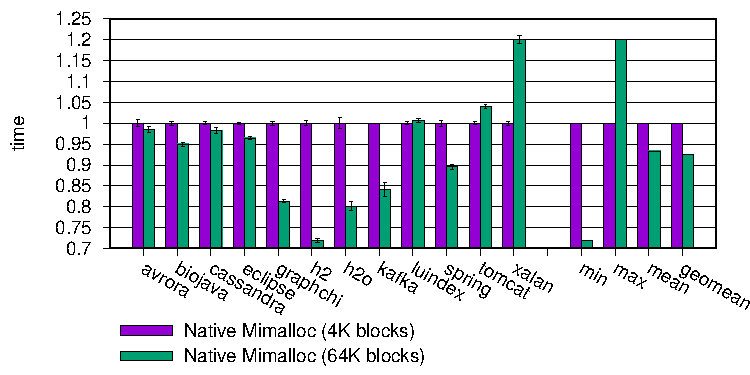
\includegraphics[width = 0.48\linewidth]{../Figures/Chopin-runbms/Chopin-runbms-time.pdf}
        \label{Chopin runbms time}
    }
    \subfloat[Mutator Time]{
        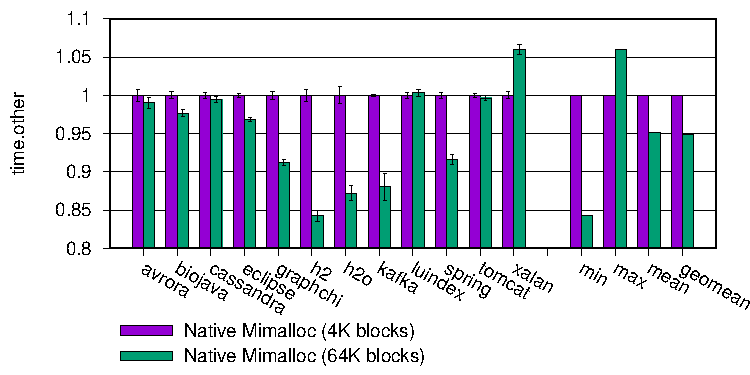
\includegraphics[width = 0.48\linewidth]{../Figures/Chopin-runbms/Chopin-runbms-mutator-time.pdf}
        \label{Chopin runbms mutator time}
    } \hfil
    \subfloat[Collector Time]{
        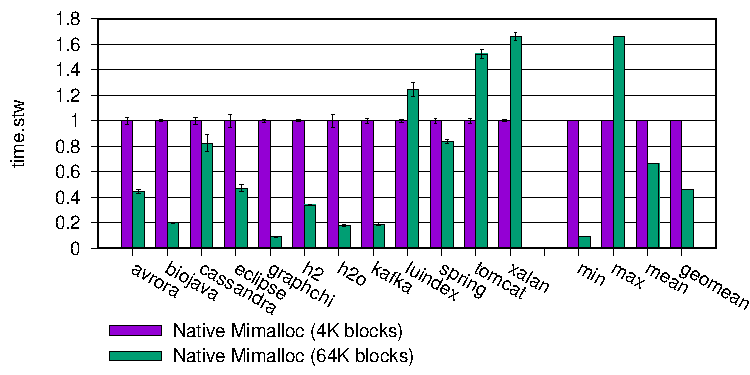
\includegraphics[width = 0.48\linewidth]{../Figures/Chopin-runbms/Chopin-runbms-collector-time.pdf}
        \label{Chopin runbms collector time}
    }
    \subfloat[GC]{
        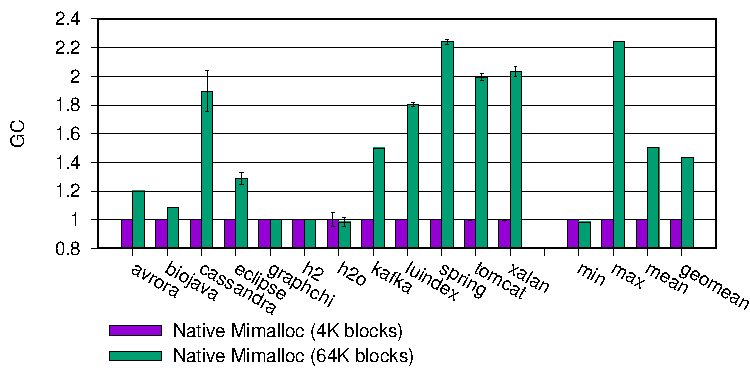
\includegraphics[width = 0.48\linewidth]{../Figures/Chopin-runbms/Chopin-runbms-GC.pdf}
        \label{Chopin runbms GC}
    }
    \caption{Chopin runbms}
    \label{Chopin runbms}
\end{figure}

\begin{figure}[H]
    \centering
    \subfloat[avrora Total Time]{
        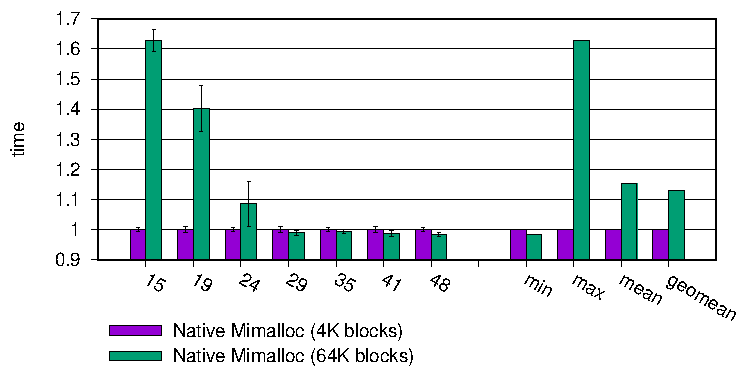
\includegraphics[width = 0.32\linewidth]{../Figures/Chopin-var-heap-size/Chopin-avrora-time.pdf}
        \label{Chopin avrora time}
    }
    \subfloat[avrora GC]{
        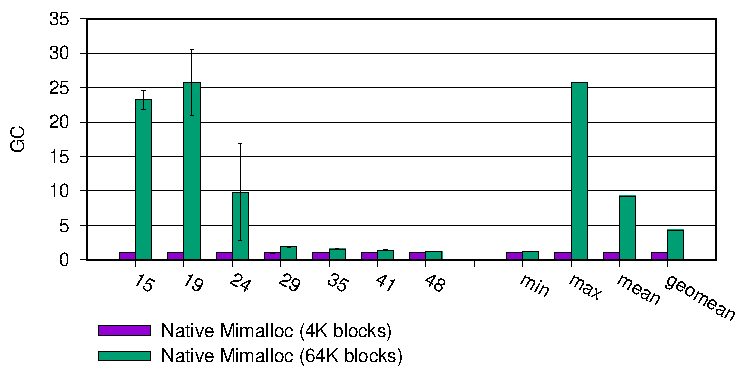
\includegraphics[width = 0.32\linewidth]{../Figures/Chopin-var-heap-size/Chopin-avrora-GC.pdf}
        \label{Chopin avrora GC}
    } \hfil
    \subfloat[luindex Total Time]{
        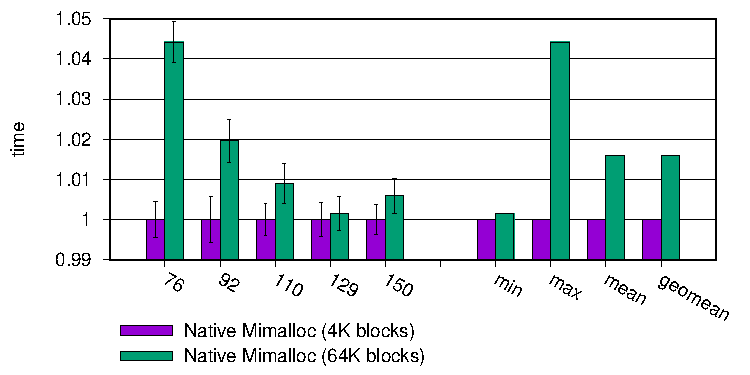
\includegraphics[width = 0.32\linewidth]{../Figures/Chopin-var-heap-size/Chopin-luindex-time.pdf}
        \label{Chopin luindex time}
    }
    \subfloat[luindex GC]{
        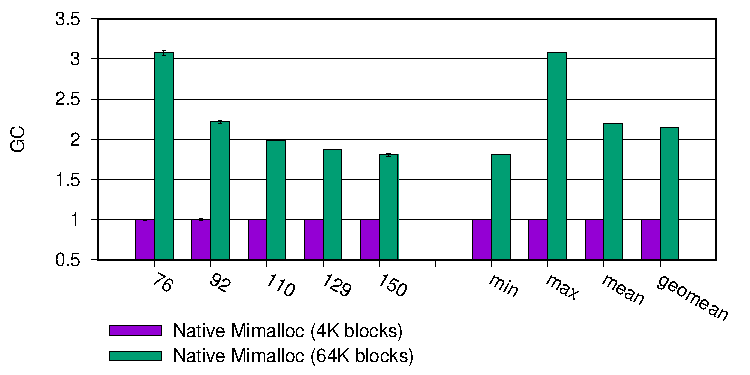
\includegraphics[width = 0.32\linewidth]{../Figures/Chopin-var-heap-size/Chopin-luindex-GC.pdf}
        \label{Chopin luindex GC}
    }
    \caption{Chopin Individual Benchmarks with Varying Heap Size}
    \label{Chopin Individual Benchmarks}
\end{figure}

\subsubsection{Bach lusearch with Various mimalloc Builds}
Note: Some of the builds are blank for smaller heap values. This is because the minheap for that particular build was greater than the heap size used for that run of the benchmark.
\begin{figure}[H]
    \centering
    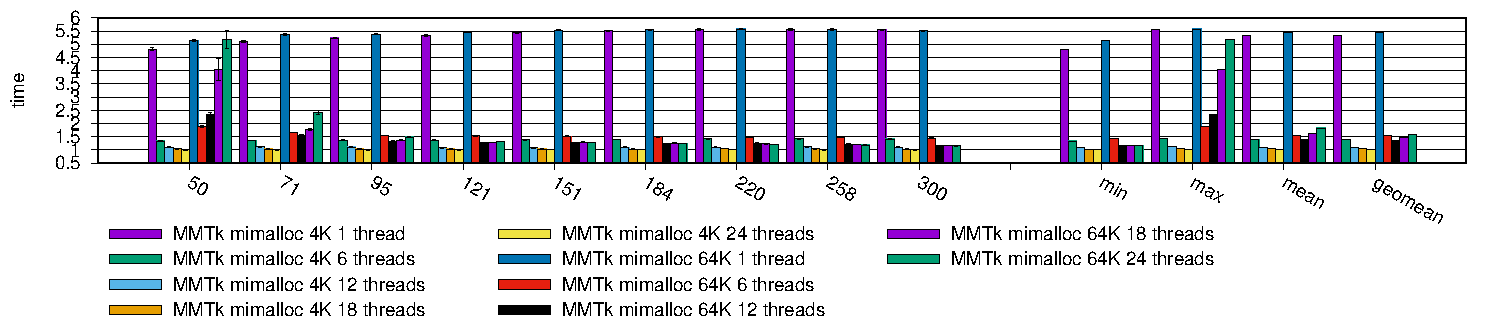
\includegraphics[scale=0.59]{../Figures/Bach-lusearch-var-threads-large-heap/Bach-lusearch-var-threads-large-heap-time.pdf}
    \caption{Bach lusearch Varying Threads time}
    \label{Bach lusearch Varying Threads time}
\end{figure}
\begin{figure}[H]
    \centering
    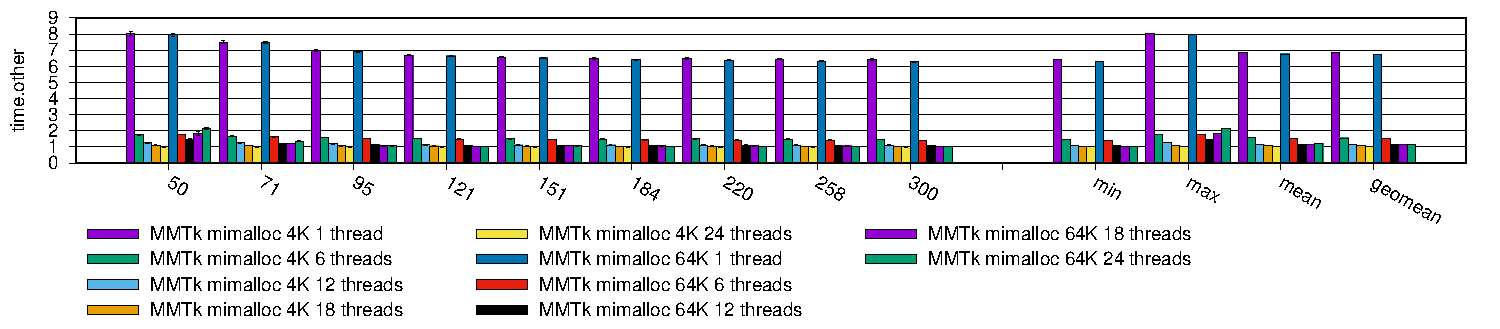
\includegraphics[scale=0.59]{../Figures/Bach-lusearch-var-threads-large-heap/Bach-lusearch-var-threads-large-heap-mutator-time.pdf}
    \caption{Bach lusearch Varying Threads mutator time}
    \label{Bach lusearch Varying Threadsmutator time}
\end{figure}
\begin{figure}[H]
    \centering
    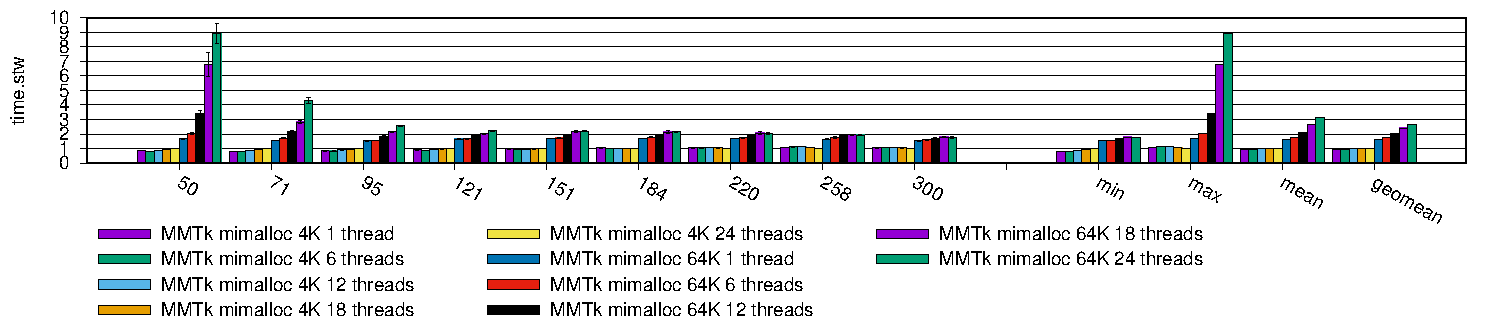
\includegraphics[scale=0.59]{../Figures/Bach-lusearch-var-threads-large-heap/Bach-lusearch-var-threads-large-heap-collector-time.pdf}
    \caption{Bach lusearch Varying Threads collector time}
    \label{Bach lusearch Varying Threads collector time}
\end{figure}
\begin{figure}[H]
    \centering
    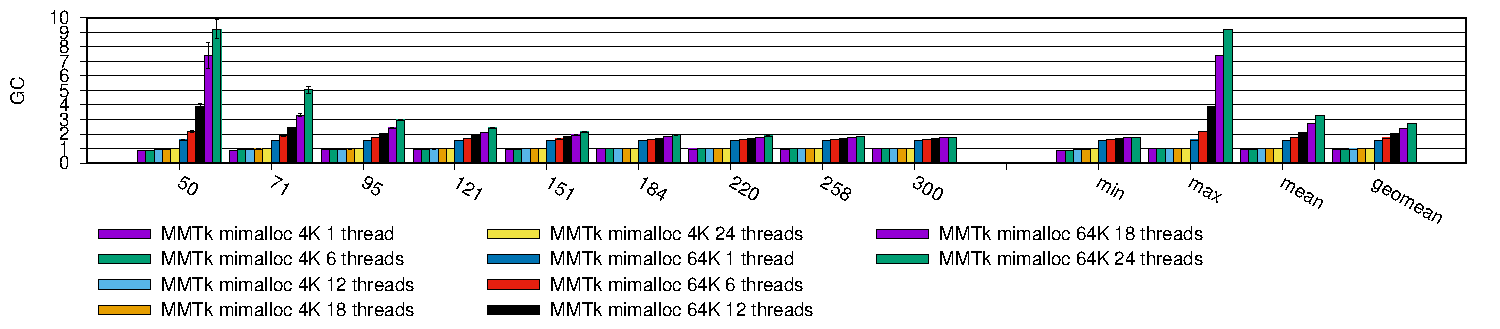
\includegraphics[scale=0.59]{../Figures/Bach-lusearch-var-threads-large-heap/Bach-lusearch-var-threads-large-heap-GC.pdf}
    \caption{Bach lusearch Varying Threads GC}
    \label{Bach lusearch Varying Threads GC}
\end{figure}

\subsubsection{Bach lusearch Varying Threads with MMTK mimalloc}
\begin{figure}[H]
    \centering
    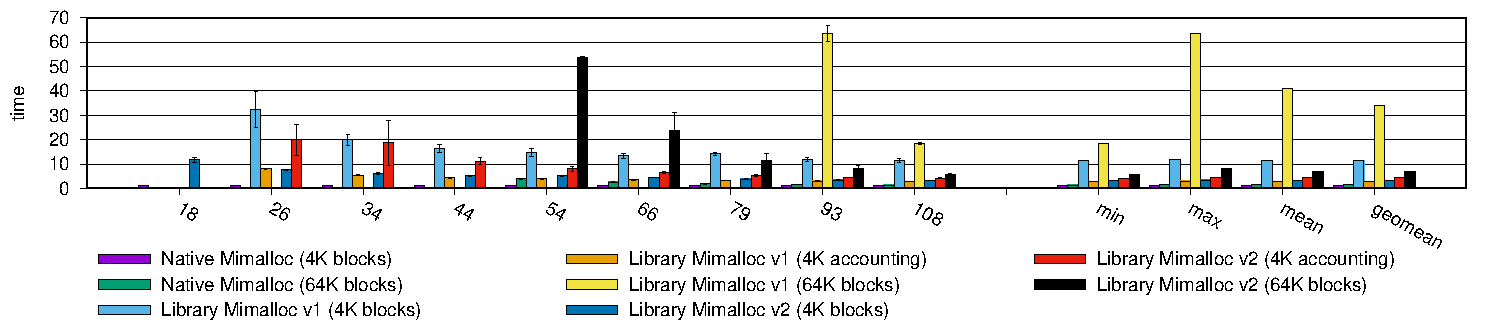
\includegraphics[scale=0.59]{../Figures/Bach-lusearch-small-heap/Bach-lusearch-small-heap-time.pdf}
    \caption{Bach lusearch time}
    \label{Bach lusearch time}
\end{figure}
\begin{figure}[H]
    \centering
    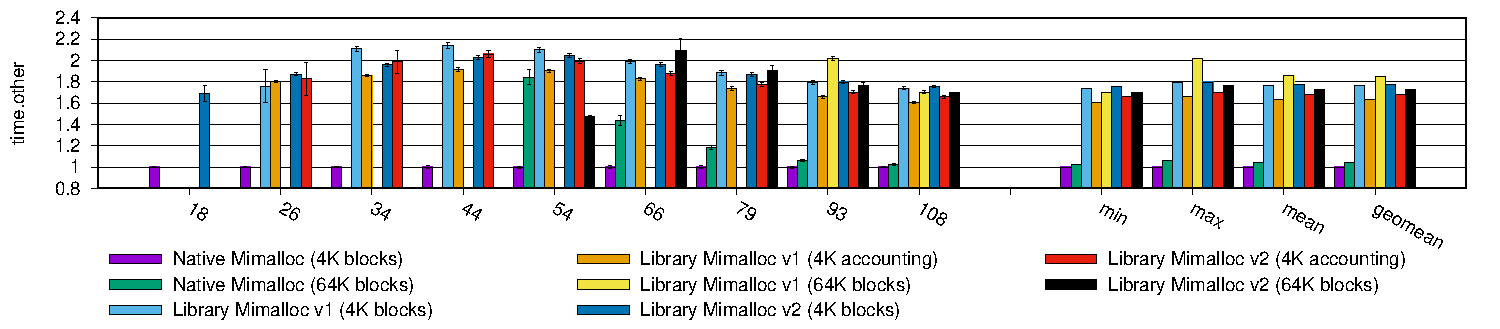
\includegraphics[scale=0.59]{../Figures/Bach-lusearch-small-heap/Bach-lusearch-small-heap-mutator-time.pdf}
    \caption{Bach lusearch mutator time}
    \label{Bach lusearch mutator time}
\end{figure}
\begin{figure}[H]
    \centering
    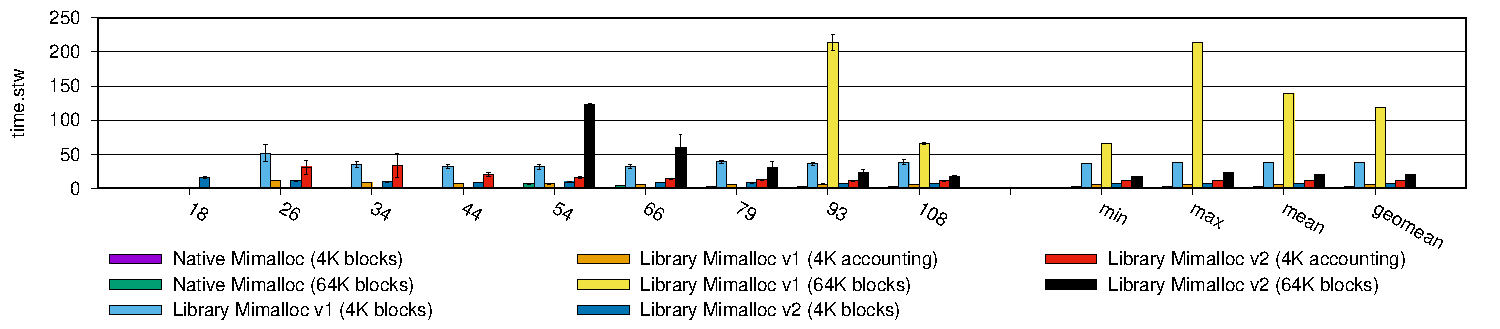
\includegraphics[scale=0.59]{../Figures/Bach-lusearch-small-heap/Bach-lusearch-small-heap-collector-time.pdf}
    \caption{Bach lusearch collector time}
    \label{Bach lusearch collector time}
\end{figure}
\begin{figure}[H]
    \centering
    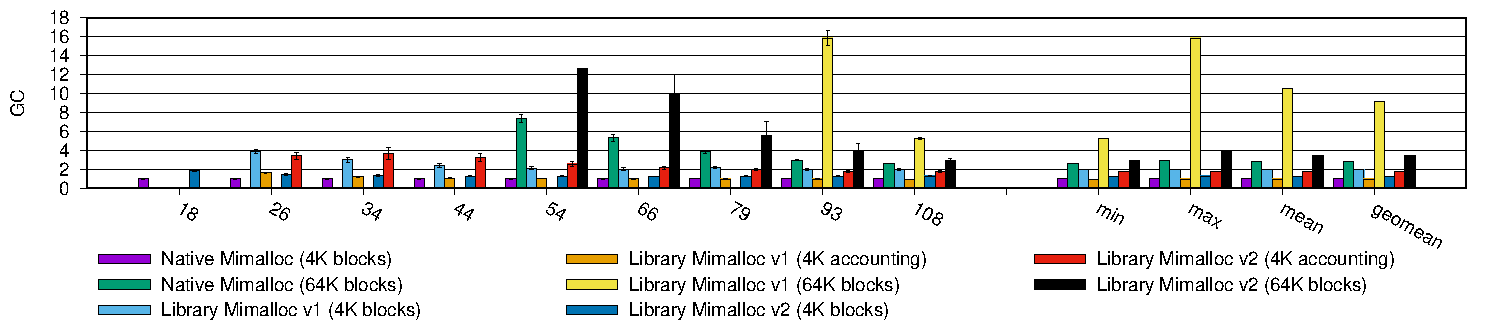
\includegraphics[scale=0.59]{../Figures/Bach-lusearch-small-heap/Bach-lusearch-small-heap-GC.pdf}
    \caption{Bach lusearch GC}
    \label{Bach lusearch GC}
\end{figure}

\subsection{Analysis}
\subsubsection{Chopin Benchmarks}
When comparing the two builds on the range of DaCapo Chopin benchmarks, the 64KiB build outperformed the 4KiB build on the majority of benchmarks, with the exceptions of luindex, tomcat and xalan. The relative geometric mean was around 0.925, a $7.5\%$ improvement in performance. It is important to note that with the heap sizes used in this run (six times the mark-compact minheap), the 64KiB build was unable to complete the fop, lusearch, pmd and sunflow benchmarks (not shown in graph), which further illustrates the space inefficiency of the design.

When considering only mutator time, the 64KiB outperformed the 4KiB on all of the benchmarks apart from luindex and xalan, with a relative geometric mean of 0.95. I expected to see these results, as the mutator time reflects the time performance of the choice of which block size to use. The interesting point here is that the geometric mean here is 0.95, higher than the geometric mean of 0.925 that I observed for the total time.

This leads us to the collector time, which acts as an indicator of spatial performance and memory efficiency, as poor memory usage will result in more collections. As expected, the 64KiB build had a substantial increase in the number of garbage collections, with a geometric mean of just over 1.4, representing an increase of over $40\%$. This matches our earlier results showing that the 64KiB build experiences severe memory fragmentation.

However, what surprised me is that despite the number of collections going up, collector time dropped substantially for the 64KiB build relative to the 4KiB build, with a geometric mean of under 0.5, representing an improvement of over $50\%$. This means that although there are more collections occurring, each one takes significantly less time. The notable exceptions to this trend were luindex, tomcat and xalan, which explains why their total time was also greater for the 64KiB build.

Although I expected the 64KiB build to outperform the 4KiB build, I did not expect the collector time to improve despite the number of collections increasing. This observation is something that the MMTk team will continue to explore.

I also ran the performance analysis over a range of heap sizes for the different benchmarks, observing that as the heap size increased, the 64KiB build performed better relative to the 4KiB build. For example, despite the 4KiB build's slightly better performance on luindex, as the heap size varied the 64KiB build performed relatively stronger, with the relative time decreasing from over 1.04 to below 1.01 as the heap size increased from 76MiB to 150MiB. Additionally, the avrora benchmark saw a decrease in relative time from over 1.6 to below 1 as the heap size increased from 15MiB to 48MiB.

This makes sense, because at a smaller heap size, when the blocks are larger, the heap will be consumed much more quickly, meaning that garbage collections will be called frequently, as demonstrated in my results. This is further exacerbated by the fact that memory is being accounted for at the block granularity for MMTk builds. We would expect that if much larger heap sizes were used, then the number of collections would go down, and the 64KiB build would perform even better relative to the 4KiB build.

My conclusion from these results is that mimalloc wants to be using 64KiB blocks over 4KiB blocks for performance purposes. However, ideally this could be attained with memory efficiency similar to that of the 4KiB block build, which may be achievable by using a finer grain of granularity for memory accounting.

\subsubsection{Bach lusearch with Various mimalloc Builds}
The performance analysis that I ran using DaCapo Bach focused primarily on lusearch compared across different builds and with varying numbers of mutator threads.

When I compared all of the mimalloc builds, it was evident that MMTk's rust implementation strongly outperforms library mimalloc, both v1 and v2. Part of the performance cost is the cost of calling the mimalloc library for every allocation, while there is also a contribution from storing metadata necessary to track the library allocations for correctness.

With the lusearch benchmark, the MMTk mimalloc build with 4KiB blocks actually outperformed the build with 64KiB blocks, although as the heap size grew, their performance became closer. With a heap size of 108MiB, the 64KiB build had a relative performance of 1.357 compared to the 4KiB build, and with a 552MiB heap, this narrowed down to 1.062. The 4KiB build's superior performance is due to having significantly fewer garbage collections. With a 108MiB heap, the 64KiB had 2.609 collections per collection for the 4KiB build.

However, it is interesting to compare the relative performance of the mimalloc v1 and mimalloc v2 builds. The mimalloc v1 build with 64KiB blocks and 4KiB accounting significantly outperformed the mimalloc v1 build with 4KiB blocks. Furthermore, recall from Section 5 that the 4KiB accounting build also was more memory efficient than the 4KiB block build, making it strongly both in memory and time performance.

mimalloc v2 surprisingly shows contrasting results. The mimalloc v2 build with 4KiB blocks outperforms the mimalloc v2 build with 64KiB blocks and 4KiB accounting. The v2 build with 64KiB blocks and 4KiB accounting also performs worse than the v1 build with 4KiB accounting, despite mimalloc v2 performing better than mimalloc v1 with the other builds.

Overall, when we compare the builds with 4KiB accounting to the builds with 64KiB accounting when using 64KiB blocks we see that they have better results not just in memory efficiency, but also in performance. This supports the idea that changing the granularity of memory accounting for MMTk mimalloc to the granularity of OS pages would substantially improve the mark-sweep collector.

\subsubsection{Bach lusearch Varying Threads with MMTk mimalloc}
I ran experiments comparing the performance of the MMTk mimalloc builds as the number of mutator threads varied from 1 to 24. At smaller heap sizes, the 64KiB build demonstrated poor scalability as its performance worsened as the number of threads increased from 6 to 24. However, this was due to the heap size being close to the minheap for 24 threads, causing an excess of collections, more than 9 times as many as the 4KiB block build with 24 threads.

However, as the heap size was increased, the 64KiB build demonstrated better temporal scalability, with the total time falling as the number of mutator threads increased. The 4KiB build similarly demonstrated this behaviour across all heap sizes.

Once again, the 4KiB build performed better than the 64KiB build, primarily due to the 64KiB build performing $50\%$ more collections, regardless of the number of threads. This further demonstrates the importance of limiting excess collections, such as by refining the granularity of memory accounting from the block granularity to the OS page granularity.

\section{Future Work}
\subsection{Further Analysis with DaCapo Chopin}
I also ran minheap experiments with DaCapo Chopin, but only for MMTk mimalloc and mimalloc v1. Below are the results for the standard 64KiB builds with 64KiB accounting:
\begin{center}
    \begin{tabular}{|l|l|l|}
        \hline
        Mutator Threads & MMTk mimalloc & mimalloc v1\\
        \hline
        1 & TIMEOUT & 108\\
        \hline
        6 & 176 & 128\\
        \hline
        12 & 226 & 130\\
        \hline
        18 & 260 & 198\\
        \hline
        24 & 287 & 222\\
        \hline
        30 & 271 & 354\\
        \hline
        36 & 280 & 450\\
        \hline
        42 & 306 & 512\\
        \hline
        48 & 307 & 660\\
        \hline
    \end{tabular}
\end{center}

Below are the linear regressions for each of the builds in the above table:
\begin{center}
    \begin{tabular}{|l|l|l|}
        \hline
        Mutator Threads & MMTk mimalloc & mimalloc v1\\
        \hline
        Gradient/Slope & 2.700 & 11.708\\
        \hline
        $y$-intercept & 191.214 & 24.603\\
        \hline
        $R^2$ & 0.8077 & 0.9301\\
        \hline
    \end{tabular}
\end{center}

Below are the results for the standard 4KiB build of MMTk mimalloc and the 4KiB accounting build for mimalloc v1:
\begin{center}
    \begin{tabular}{|l|l|l|}
        \hline
        Mutator Threads & MMTk mimalloc & mimalloc v1\\
        & 4KiB blocks & 4KiB accounting\\
        \hline
        1 & 41 & 59\\
        \hline
        6 & 44 & 64\\
        \hline
        12 & 45 & 64\\
        \hline
        18 & TIMEOUT & 67\\
        \hline
        24 & 46 & 65\\
        \hline
        30 & 47 & 73\\
        \hline
        36 & 46 & 77\\
        \hline
        42 & 44 & 81\\
        \hline
        48 & 48 & 89\\
        \hline
    \end{tabular}
\end{center}

Below are the linear regressions for each of the builds in the above table:
\begin{center}
    \begin{tabular}{|l|l|l|}
        \hline
        Mutator Threads & MMTk mimalloc & mimalloc v1\\
        \hline
        Gradient/Slope & 0.0904 & 0.5708\\
        \hline
        $y$-intercept & 42.8773 & 57.2378\\
        \hline
        $R^2$ & 0.5143 & 0.9081\\
        \hline
    \end{tabular}
\end{center}

The results from Chopin were quite surprising. In particular, the slope for mimalloc v1 was higher than my estimation accounted for. It would be good to run further experiments on Chopin in the future.

\subsection{MMTk mimalloc Development}
\subsubsection{Granularity of Memory Accounting in MMTk mimalloc}
As discussed earlier, following the minheap and performance results, I hypothesised that a build of MMTk mimalloc with 64KiB blocks that only commits memory at the OS page granularity will be able to represent the best of both worlds in regards to this tradeoff.

The idea is that we would see memory efficiency very similar to the 4KiB block build, which was comparable to the memory efficiency of MarkCompact, but with the improved performance of the 64KiB block build. Furthermore, based on how 4KiB accounting builds of library mimalloc outperformed 64KiB accounting builds of the same mimalloc version, we would expect the performance to be improved even further, making a much more competitive allocator.

A similar idea may also be implemented in MMTk's Immix collector \cite{blackburn2008immix,mmtk-core}, which similarly accounts for memory at the granularity of its 32KiB blocks. Immix does not suffer from the pathological memory usage increases that mimalloc does, since it does not have 48 distinct size classes with its blocks \cite{blackburn2008immix}, but this may still represent a marginal improvement, and increase consistency among MMTk's framework.

\subsubsection{Hard-Coded Aspects of MMTk mimalloc}
In order to run experiments on builds of MMTk's implementation of Rust with different block sizes, I made a small change to the codebase. Previously, the maximum large object size was defined as a constant. However, when producing builds with a different block size, this would result in an error due to the allocator attempting to allocate objects larger than the blocks they are being allocated to. In order to enable the production of builds with different block sizes, I replaced this constant with a variable size matching the block size to avoid this error \cite{pr747}.

Something for future consideration with MMTk mimalloc would be modifying the sizes of the bins to reflect changes like this as well, as they remained hard-coded \cite{mmtk-core}. For builds with a smaller block size, multiple bins would remain empty, since their object size was larger than the block size. This would make it easier to evaluate different block sizes with MMTk mimalloc in the future.

\subsubsection{mimalloc v2}
Another consideration is upgrading to mimalloc v2, which uses a new algorithm for organising internal mimalloc blocks in order to reduce memory usage and fragmentation compared to mimalloc v1 \cite{mimalloc}. This is supported by my results with the lusearch benchmark. However, further evaluation, both of memory efficiency and performance analysis, will be required before upgrading the MMTk port of mimalloc.

\section{Related Work}
\subsection{Huge Pages}
Huge OS pages are being used with increasing frequency in order to reduce stress on the TLB, allowing each entry to cover a much larger region of memory. A relevant example is Temeraire, a hugepage-aware extension to tcmalloc following the idea that `malloc can get slower, while the program gets faster'. It uses hugepages (2MiB) from the OS rather than the standard 4KiB pages, and focuses on reducing fragmentation and stress on the TLB \cite{hunter2021beyond}.

In the Teremaire paper, it is suggested that mimalloc could also benefit from a similar hugepage-aware allocator, although the fact that mimalloc segments are maintained per-thread makes it more difficult to perform dense bin-packing in a similar manner to Teremaire \cite{hunter2021beyond}.

\subsection{minheap Determinism}
Steve Blackburn from MMTk has recently been investigating the determinism of minheap experiments using the DaCapo Chopin versions of the fop, lusearch, cassandra and eclipse benchmarks. Initially, the assumption had been that these experiments were deterministic, but the results from Steve's experiments contradict this. Across three trials with the same configs, fop had stable minheap results, but lusearch, cassandra and eclipse showed some variation. Cassandra showed the most variation with up to $4\%$ variation \cite{dacapo-repo}.

While these results indicate that there is some variation in the minheap of some benchmarks, the variance may not be very significant. There is room for further investigation in this area.

\section{Conclusion}
mimalloc is a modern allocator that aims to improve spatial locality, and balance the simultaneous demands of concurrency, performance, security and memory efficiency, through the implementation of free list sharding. MMTk, a framework for implementing memory managers, has an implementation of mimalloc as the allocator for its mark sweep collection plan. Initial testing demonstrated unexpected increases in the minheap for mimalloc as the number of mutator threads increased. Through two sets of experiments run using DaCapo benchmarks, two problems were identified in the MMTk codebase. The first problem was related to MMTk's memory accounting when using library mimalloc, which should be at the OS page granularity. This was addressed in a pull request resulting from the project. The second problem was related to MMTk's Rust implementation of mimalloc, which commits each 64KiB block instead of at the page granularity in a similar way to library mimalloc. Addressing this problem is the next step for MMTk's analysis of the mark sweep collector. I also ran performance analysis experiments comparing various builds of mimalloc, concluding that MMTk's implementation had superior performance, and that the builds with 64KiB blocks outperformed the builds with 4KiB blocks.

\section*{Acknowledgements}
I would like to thank Steve Blackburn and the MMTk team at ANU for their help and guidance throughout this project.

\bibliographystyle{plain}
\bibliography{bibliography}
\end{document}